\chapter{Quá trình xử lý dữ liệu BVH}
\label{Appendix2}

\section{Cấu trúc tệp dữ liệu BVH}

File BVH (Biovision Hierarchy) là một định dạng file dữ liệu chứa thông tin về cấu trúc xương và dữ liệu về chuyển động của xương trong một hệ thống xương. File BVH bao gồm hai phần chính: phần khai báo cấu trúc xương và phần dữ liệu chuyển động của xương. 
%Mỗi phần được phân cách bởi từ khóa \texttt{MOTION}.

\setcounter{figure}{15}
\begin{figure}
	\centering
	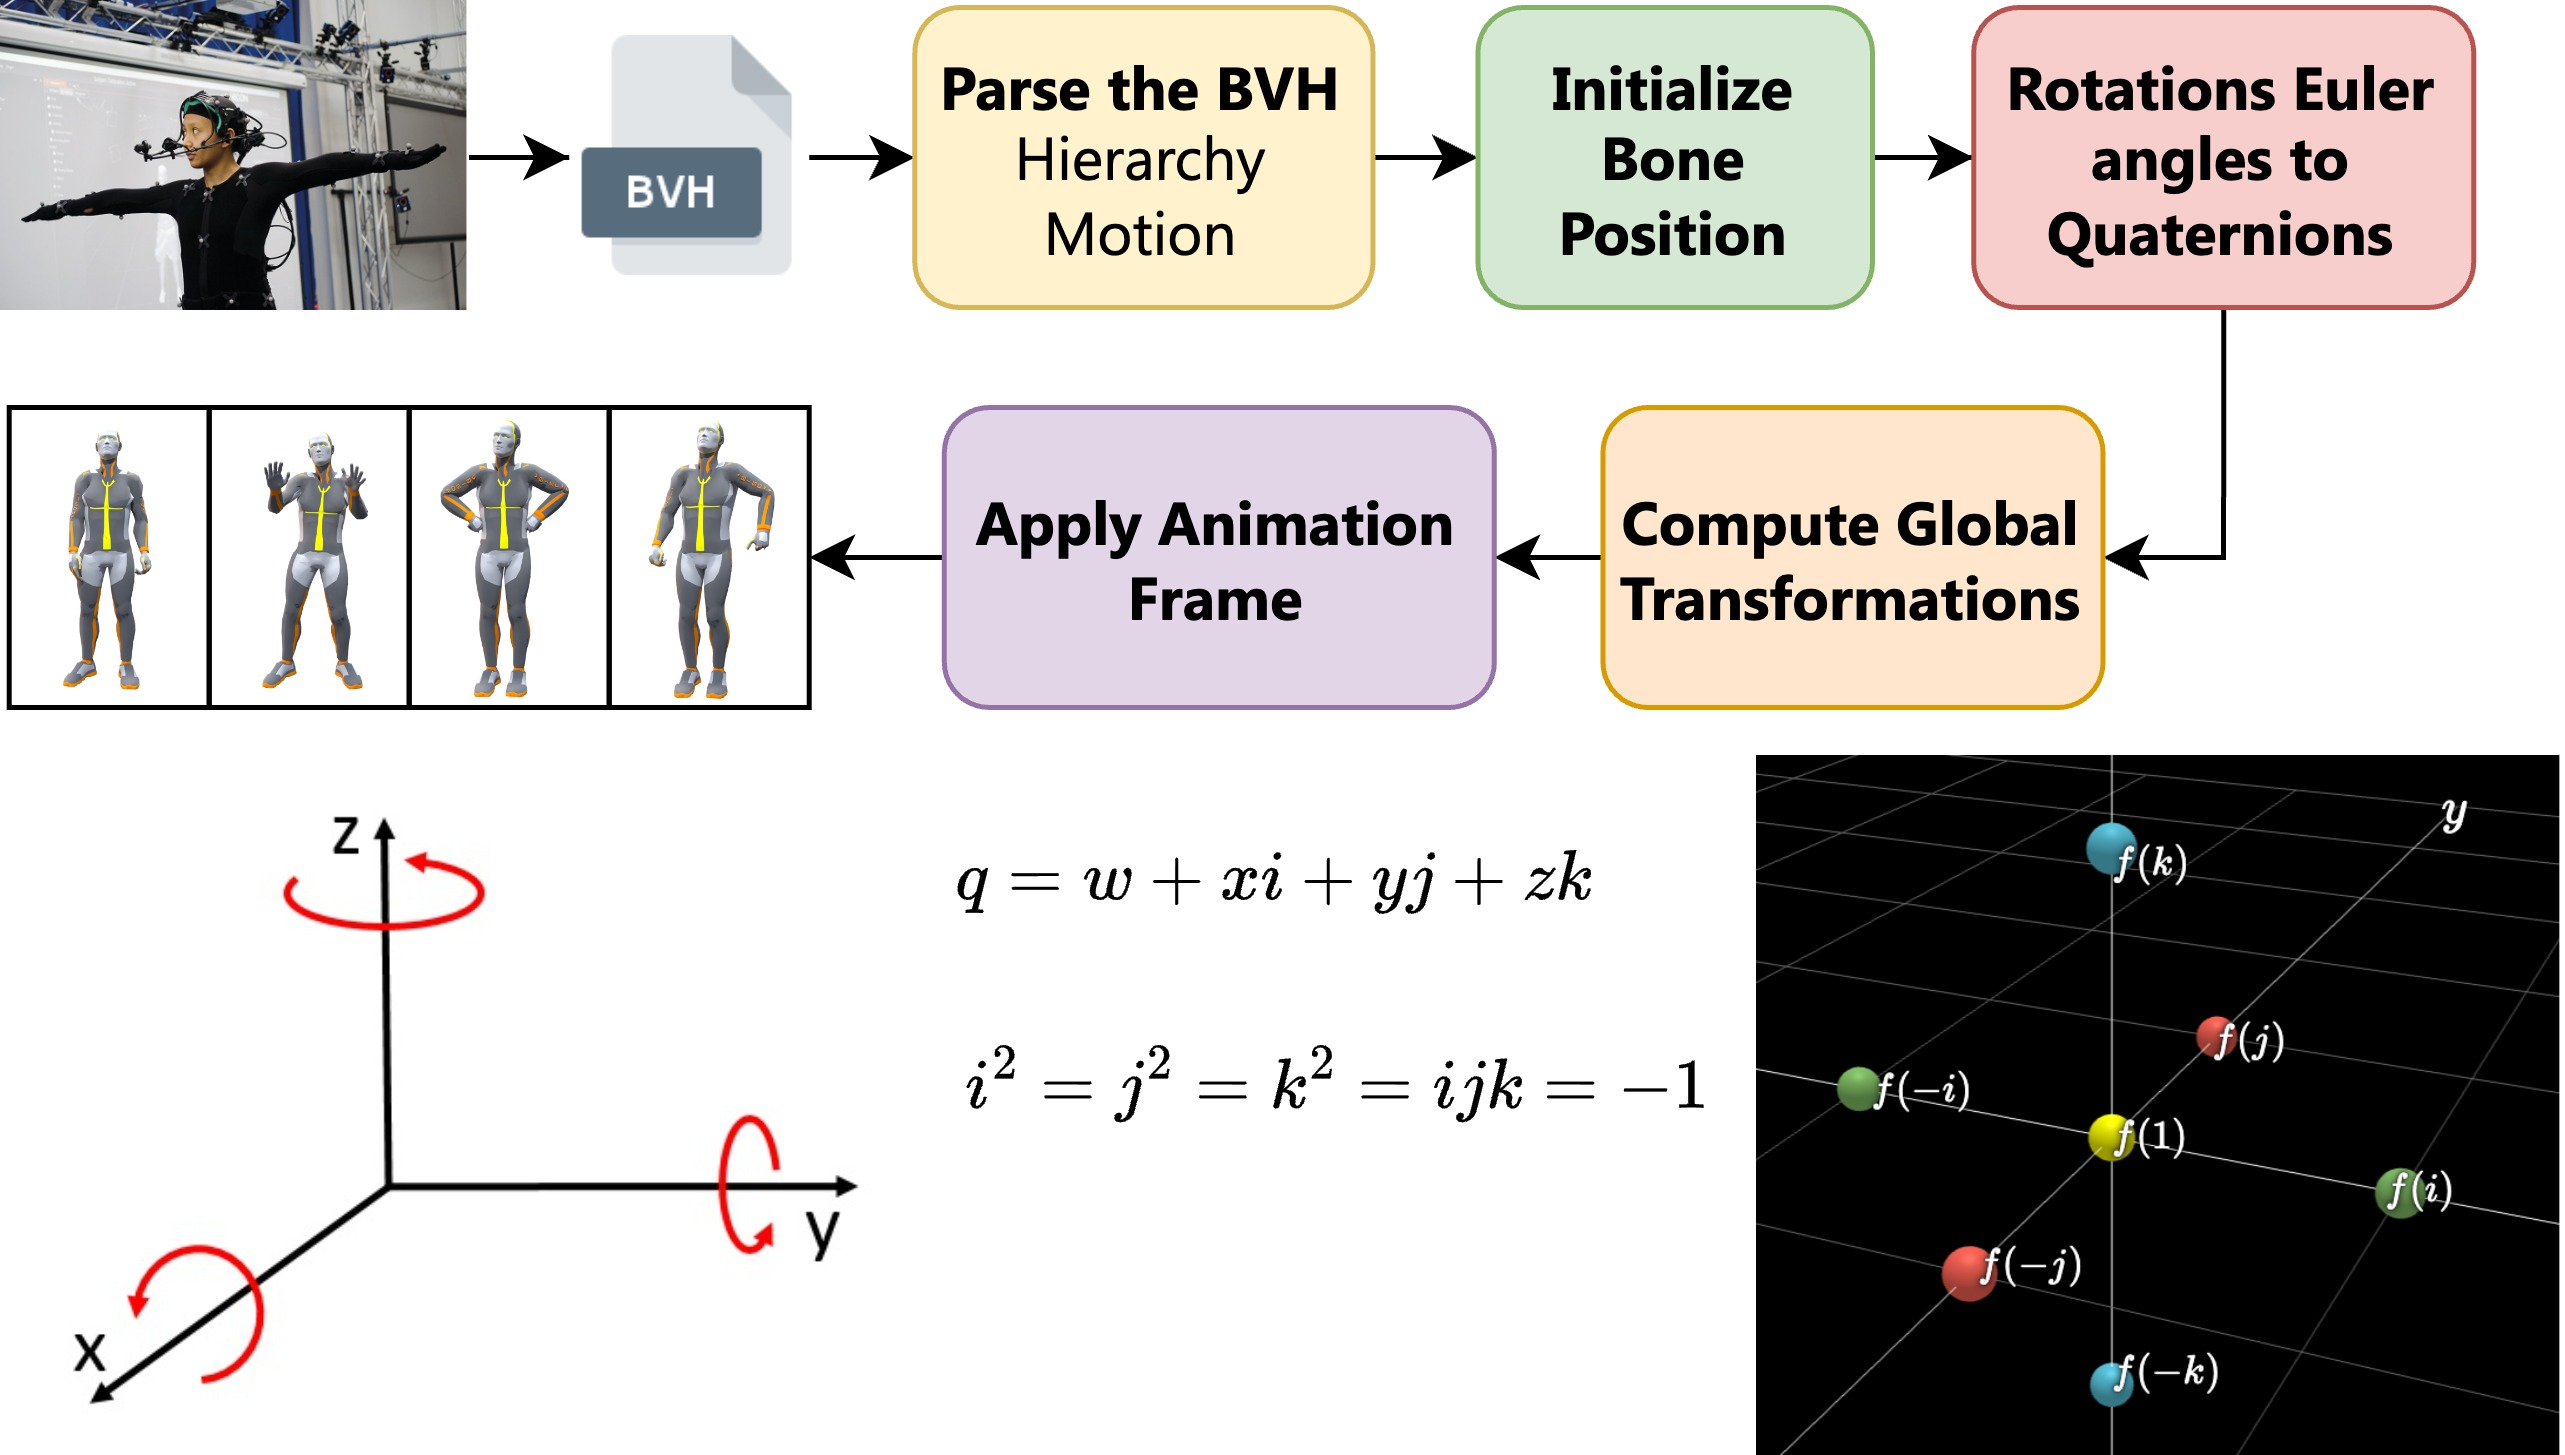
\includegraphics[width=\linewidth]{BVH}
	\caption{Quá trình xử lý tệp tin BVH}
	\label{fig:BVH}
\end{figure}


	\textbf{Hierachy}: bao gồm 75 Bone $\{ \mathbf{t}_i \}^{75} $, có vị trí ban đầu  $\mathbf{t}_{i} = \{t_x, t_y, t_z\}$

\vspace{5pt}

\textbf{Motion}:
Bone trong dữ liệu BVH bao gồm vị trí $\mathbf{position}_{\operatorname{local}}  \in \mathbb{R}^{3}$ và góc quay $\mathbf{rotation}_{\operatorname{local}} \in \mathbb{R}^{3}$.
%	\begin{figure}
	%		\centering
	%		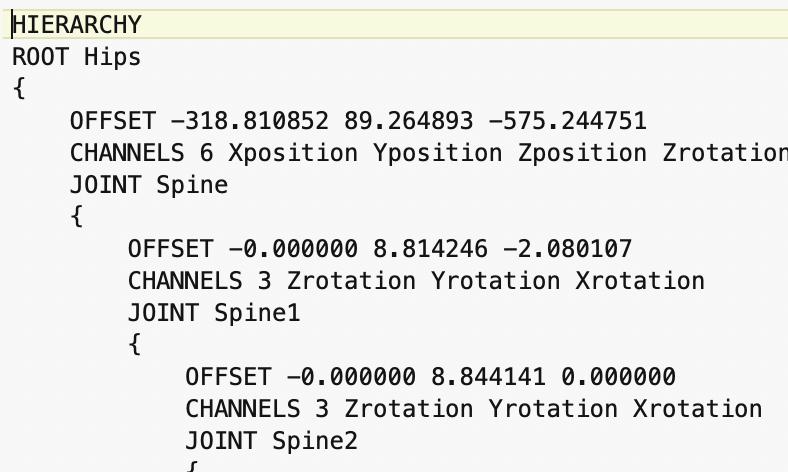
\includegraphics[width=0.25\textwidth]{BVHFile}
	%	\end{figure}
$\mathbf{rotation}_i^{\operatorname{local}} = \{ \alpha ,\beta , \gamma \}$ lần lượt là góc quay quanh các trục $Z$ ,$Y$ , và $X$, góc quay tổng hợp ba trục trong không gian Eule là $R = R_Z(\alpha) R_Y(\beta) R_X(\gamma)$.
Để tính toạ độ chuyển động của một nhân vật, ta thực hiện phép toán sau:

\begin{equation}
	\mathbf{position}_{\text{global}} = R \cdot \mathbf{position}_{\text{local}} + \mathbf{t}
\end{equation}


\section{Quá trình chuyển góc quay Euler sang Quaternion}

%Quaternion là một cách biểu diễn góc quay trong không gian ba chiều. Quaternion có dạng $q = a + bi + cj + dk$, trong đó $ư, b, c, d$ là các số thực. Quaternion có thể được biểu diễn dưới dạng ma trận $4 \times 4$ như sau:


Để tránh Gimbal lock, ta phải chuyển dữ liệu ở dạng góc quay Euler sang dạng góc quay Quaternion. Trong đó góc quay từng Bone dạng Euler ZYX sang dạng Quaternion, mỗi Bone biểu diễn bằng 4 phần tử $q = (q_w, q_x, q_y, q_z)$, với các giá trị được tính như sau:
%	Mỗi Bone được biểu diễn thành: 
%	$$q = w + xi + yj + zk$$
%	c
%	$$i^2 = j^2 = k^2 = ijk = -1$$

Đầu tiên, chúng ta tính các giá trị $\cos$ và $\sin$ của một nửa góc quay cho mỗi trục:


\begin{itemize}
	\item $c_{\alpha} = \cos\left(\frac{\alpha}{2}\right), \quad s_{\alpha} = \sin\left(\frac{\alpha}{2}\right)$
	\item $c_{\beta} = \cos\left(\frac{\beta}{2}\right), \quad s_{\beta} = \sin\left(\frac{\beta}{2}\right)$
	\item $c_{\gamma} = \cos\left(\frac{\gamma}{2}\right), \quad s_{\gamma} = \sin\left(\frac{\gamma}{2}\right)$
\end{itemize}

Dựa trên các giá trị tính được ở trên, các thành phần của quaternion được tính như sau:


\begin{itemize}
	\item $q_w = c_{\alpha} c_{\beta} c_{\gamma} + s_{\alpha} s_{\beta} s_{\gamma}$
	\item $q_x = c_{\alpha} c_{\beta} s_{\gamma} - s_{\alpha} s_{\beta} c_{\gamma}$
	\item $q_y = c_{\alpha} s_{\beta} c_{\gamma} + s_{\alpha} c_{\beta} s_{\gamma}$
	\item $q_z = s_{\alpha} c_{\beta} c_{\gamma} - c_{\alpha} s_{\beta} s_{\gamma}$
\end{itemize}

Với quaternion $q$ đã tính, vị trí toàn cục của bone $\mathbf{p}_{\text{global}}$ được xác định bằng cách quay vị trí cục bộ $\mathbf{p}_{\text{local}}$ thông qua công thức:

\begin{equation}
	\mathbf{p}_{\text{global}} = q \cdot \mathbf{p}_{\text{local}} \cdot q^{-1} + \mathbf{t}
\end{equation}

với $\mathbf{t}$ là vị trí gốc của bone trong không gian toàn cục.



